\documentclass{beamer}
\usepackage{graphicx,mathtools,mathpartir}
\usepackage{hyperref}
\usepackage{tikz}
\usetikzlibrary{positioning}
%\setbeamertemplate{caption}{\raggedright\insertcaption\par}
%\setbeamerfont{caption}{size=\scriptsize}
\useoutertheme{infolines}
\setbeamertemplate{navigation symbols}{}
% \setbeamertemplate{bibliography item}{[\theenumiv]}

\AtBeginSection{\frame{\sectionpage}}
\AtBeginSubsection{\frame{\subsectionpage}}

\defbeamertemplate{section page}{mine}[1][]{%
  \begin{centering}
    %{\usebeamerfont{section name}\usebeamercolor[fg]{section name}#1}
    %\vskip1em\par
    \begin{beamercolorbox}[sep=12pt,center]{part title}
      \usebeamerfont{section title}\insertsection\par
    \end{beamercolorbox}
  \end{centering}
}

\defbeamertemplate{subsection page}{mine}[1][]{%
  \begin{centering}
%    {\usebeamerfont{subsection name}\usebeamercolor[fg]{subsection name}#1}
%    \vskip1em\par
    \begin{beamercolorbox}[sep=8pt,center,#1]{part title}
      \usebeamerfont{subsection title}\insertsubsection\par
    \end{beamercolorbox}
  \end{centering}
}
\setbeamertemplate{section page}[mine]
\setbeamertemplate{subsection page}[mine]

\title[]{Introduction to My Current and Future Work}
\author[]{Krzysztof Drewniak}
\institute[]{Visiting student at HPAC}
\date[]{4 Oct 2017}

\begin{document}
\begin{frame}[plain]
\titlepage{}
\end{frame}

\begin{frame}
  \frametitle{Outline}
  \tableofcontents{}
\end{frame}

\section{About Me}
\begin{frame}
  \frametitle{Why I'm Here}
  \begin{itemize}
  \item Bachelor's student in Computer Science and (Pure) Mathematics at the University of Texas at Austin
  \item Degree almost complete --- need to write and defend research thesis to graduate with honors
  \item Invited by Prof.\ Bientinesi to work on Linnea project
  \item Will be staying at RWTH from September to mid-January
  \end{itemize}
\end{frame}

\begin{frame}
  \frametitle{Research Background}
  \begin{itemize}
  \item Computational epidemiology with Dr.\ Armin R.\ Mikler at U. of North Texas while in early college high school
    \begin{itemize}
    \item Worked on how to reduce epidemic spread
    \item Vaccination strategies based on centrality (in the graph that served as a model)
    \end{itemize}
  \item Joined Dr.\ Robert Van De Giejn's group at UT Austin last year
    \begin{itemize}
    \item Was initially interested in FLAME
    \item Created an algorithm for $D += ABC$
    \end{itemize}
  \item Interests are in the intersection of program correctness and low-level systems programming
  \end{itemize}
\end{frame}

\begin{frame}
  \frametitle{Industry Background}
  Last four summers were spent doing internships:
  \begin{itemize}
  \item Google Summer of Code ---  adding more thorough Unicode support to a Lisp implementation
  \item WhatsApp --- Server-side media handling improvements and some encryption things
  \item TrueCar --- Machine learning (that is, database scouring) for fake-order detection
  \item Microsoft, Bing Maps --- Deep learning to improve maps suggestions
  \end{itemize}
\end{frame}

\section{\texttt{gemm3()}}
\begin{frame}
  \frametitle{Problem}
  \begin{itemize}
  \item Want to compute $D += ABC$
  \item If we only have \texttt{gemm()} (or \texttt{trmm()} $\ldots$), need to break into
    \begin{align*}
      T &= BC\\
      D &+= AT\\
    \end{align*}
  \item $T$ is often large, causing memory consumption issues
  \item Writing to/from memory can also be costly
  \end{itemize}
\end{frame}

\begin{frame}
  \frametitle{Solution}
  \begin{itemize}
  \item New algorithm to compute $D += A(BC)$ in constant memory
  \item Uses two different matrix multiply algorithms
  \item Inner algorithm is called to compute at most cache-sized blocks of $(BC)$
  \item Reduces memory impact by never storing all of $(BC)$
  \item Also increases performance by keeping intermediates in cache
  \end{itemize}
\end{frame}

\begin{frame}
  \frametitle{Memory results}
  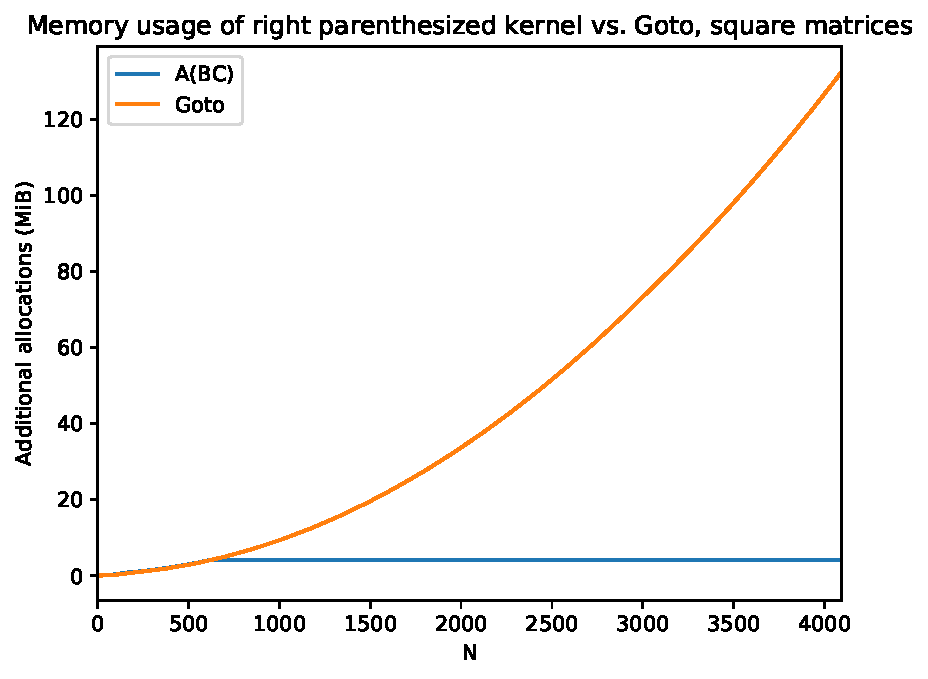
\includegraphics[height=0.9\textheight]{right-paren-memory}
\end{frame}

\begin{frame}
  \frametitle{Performance results}
  4.7\% GFlops/s higher for square matrices (5.1\% in left-parenthesized case)
  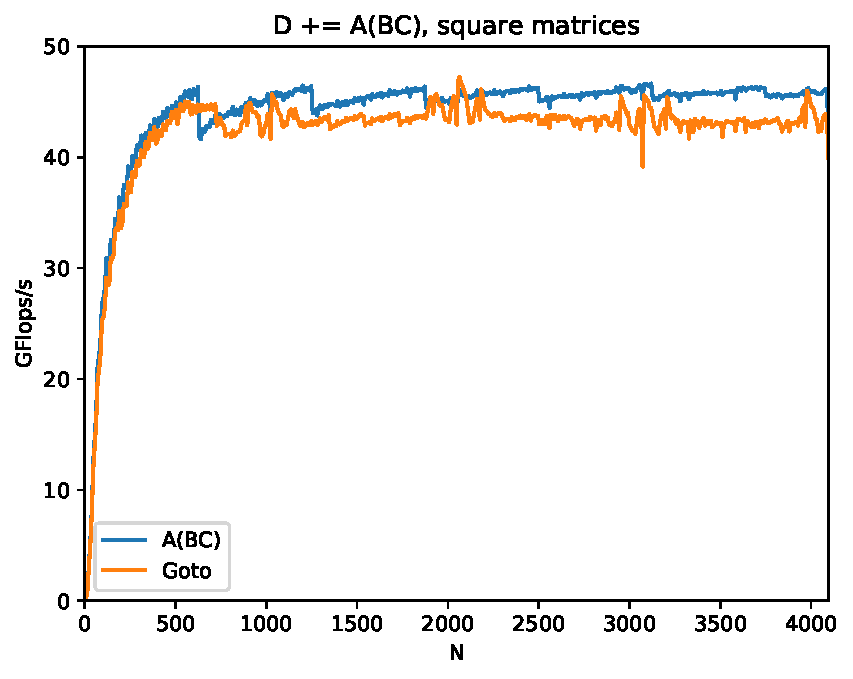
\includegraphics[height=0.9\textheight]{right-paren-plot}
\end{frame}

\section{Simplifying Expressions in Linnea}
\begin{frame}
  \frametitle{Overview of Linnea}
  \begin{itemize}
  \item Compiles linear algebra expressions into series of BLAS/LAPACK calls
  \item Generates code which significantly outperforms other systems
  \item Operates on symbolic expressions
  \begin{center}
    \begin{tikzpicture}[grow=down, thick]
      \node (e) {$A(B + C)$};
    \node [right= 2cm of e] (t1) {$\times$}
    child {
      node {$A$}
      edge from parent
    }
    child {
      node {$+$}
      child {
        node {$B$}
        edge from parent
      }
      child {
        node {$C$}
        edge from parent
      }
      edge from parent
    };
    \path (e) -- node {$\equiv$} (t1);
  \end{tikzpicture}
\end{center}
\item Simplifying expressions is central to Linnea

  Ex. $ABB^{-1} \to AI \to A$
\end{itemize}
\end{frame}

\begin{frame}
  \frametitle{Simplifying expressions in Linnea}
  \begin{itemize}
  \item Linnea needs to simplify expressions in order to check their equivalence and correctly apply kernels
  \item The simplification rules are based on linear algebra identities
    \begin{itemize}
    \item $\alpha A + \beta A \to (\alpha + \beta) A$
    \item $A^T \to A$ (only when $A$ is symmetric)
    \end{itemize}
  \item Simplification code is currently handwritten, requiring much time and effort
  \end{itemize}
\end{frame}

\begin{frame}
  \frametitle{Goal}
  \begin{itemize}
  \item Find a way to autogenerate the simplification module for Linnea
  \item Benefits:
    \begin{itemize}
    \item Requires only knowledge of the underlying identities
    \item Less hand-written code, so fewer bugs
    \item Generalizability --- same code could be used for a tensor compiler or similar
    \item Potentially improved performance
    \end{itemize}
  \end{itemize}
\end{frame}

\begin{frame}
  \frametitle{Generating term rewriting systems}
  \begin{itemize}
  \item Term rewriting systems are a set of rewrite rules that operate on algebraic expressions
  \item Pattern matching identifies applicable rules
  \item Algorithms exist to turn sets of identities into rewrite systems that produce a normal form
    \begin{itemize}
    \item Main example: Knuth-Bendix algorithm
    \end{itemize}
  \item Do not always succeed or even terminate
  \item Not known to handle constraints (like $A = A^T$ if $A$ is symmetric)
  \end{itemize}
\end{frame}

\begin{frame}
  \frametitle{Plan}
  \begin{itemize}
  \item Adapt Knuth-Bendix (or similar) algorithms for this purpose and implement them
    \begin{itemize}
    \item If this fails, investigate other potential techniques for this problem
    \end{itemize}
  \item Translate known identities into rewrite system
  \item Generate efficient simplification code based on rewrite rules
  \end{itemize}
\end{frame}
\end{document}
